% !TEX root = ../main.tex
\section{Psychology and Human Factors}\label{sec:humanfactors}

	In many years, the field of psychology have been important in order to understand how humans interpret and remember information. Psychology studies have recognized that the human brain have a superior memory for remembering and recalling visual information rather than recognizing and recalling verbal or textual information \cite{DeAngeli}. To be able to go beyond the technical part of security, this section includes related work on passwords focusing on psychology and the human aspects. Combining research from the two different disciplines computer security and psychology, can give a deeper understanding of passwords at a human level.

		\begin{wrapfigure}{r}{0.4\textwidth}
      \vspace{-10pt}
      \begin{center}
        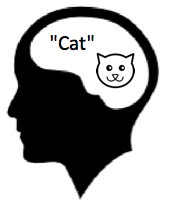
\includegraphics[scale=0.5]{pics/review/dualCoding.png}
      \end{center}
      \vspace{-10pt}
      \caption{Dual-Coding Theory}
      \vspace{-10pt}
      \label{fig:dualcoding}
    \end{wrapfigure}

	One known theory from the world of psychology is the {\it dual-coding theory} \cite{Biddle}. The theory suggests that verbal and non-verbal memory are processed and represented differently in humans mind. Text are verbal information represented by symbols, in contrast to non-verbal information like images that mentally represent perceived concepts assigned to a perceived meaning of what is being directly observed. Both verbal and non-verbal information can be used when recalling information. For example, a person have received stimulus of the concept {\it cat}, the image as well as the word {\it cat} (Figure~\ref{fig:dualcoding}). When a person is asked to recall the concept of {\it cat}, a person can retrieve the image or the word individually, or both simultaneously. If a person remembers the word {\it cat}, the image of the cat is not lost will be possible to retrieve at a later point in time. The ability to code a stimulus in two separate ways can increase human's ability to remember, in contrast to only code the stimulus one way.

	When it comes to humans and visual interpretation, studies support the idea that people recall symmetric images better than asymmetric images \cite{Attneave, French}. A particular interesting observation is that mirror symmetry carries a special status I the human memory \cite{Wagemans1}. An understanding of psychological studies on visual memory can help to build successful attacks against graphical passwords. If an attacker successfully manages to use the symmetric properties of graphical password schemes, the security of the scheme might be significantly reduced.

  Besides choosing symmetric password, humans tend to be influenced by graphical elements in a password scheme. A study on the {\it PassFace} scheme \cite{Davis} revealed that there was a high bias in the password selection according to a user's gender and race. When analyzing the choice of faces according to the participant's gender, most of the male and female participants chose female faces. In addition to the bias towards preferring female faces, 60-70\% of the participants preferred a model over a typical female/male person. They also looked at the race of the faces, where the results showed that almost all of the participant preferred their own race. This research raises the question if it is possible to analyze user's choice in passwords based on the demographics of a user.

  A difference in graphical and text-based password schemes is that graphical passwords can use images with colors that may influence a user's choice in graphical passwords. In a user-study \cite{Thorpe2} on the image-based scheme {\it PassPoints}, it was observed that different images were easier guessed compared to other pictures. When analyzing different images and visualizations, gestalt psychology \cite{Wagemans2} is an important field to understand user's interpretation of visual objects. The picture from the user-study being easily guessed was the picture of cars in various positions and different colors. A possible explanation could be that humans seek to find a pattern in an image that are easily remembered. Structured images can be analyzed by using the principles of grouping, similarities of color, and similarity of size in the picture, e.g. the gestalt principles, helping humans to be able to remember the image.

  Password habits may be different across different subpopulation as a cause of background and culture. In 2012, Joseph Bonneau released an analysis of 70 million passwords from {\it Yahoo!} \cite{Bonneau2}. The passwords were analyzed in terms of guessing rate by performing a dictionary attack. The collected data contained 328 subpopulations. The results showed that there were no better populations compared to others in the collected data, but there was observed a variation in the different populations. Demographically, gender had a small effect on the guessing rate while age increased across different age groups. The analysis also revealed that language had a significant impact on the password strength where Indonesian-speaking users were among the weakest subpopulations as a contrast to German and Korean-speaking users that provided stronger passwords.

	